\begin{frame}
  \frametitle{Задача <<Гонка со временем>>}
  \begin{center}
    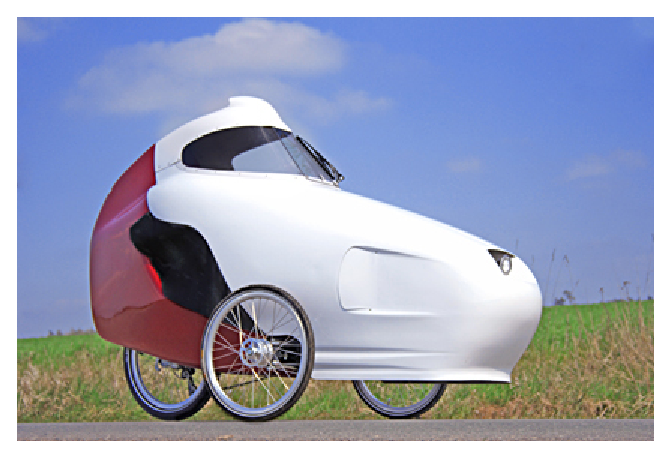
\includegraphics{race-1.eps}
  \end{center}
\end{frame}

\begin{frame}
  \frametitle{Над задачей работали}
  \begin{itemize}
    \item Идея задачи: Юрий Петров
    \item Текст условия: Сергей Поромов
    \item Тесты, проверяющая программа и др.: Юрий Петров
    \item Решения: Юрий Петров, Сергей Поромов
    \item Текст разбора: Юрий Петров
  \end{itemize}
\end{frame}

\begin{frame}
  \frametitle{Формулировка задачи}
  \begin{itemize}
    \item
      Школьники
      \begin{itemize}
        \item Представлены точками на прямой
        \item Движутся к точке $0$
        \item Движутся с постоянными скоростями
      \end{itemize}
    \item
      Веломобиль
      \begin{itemize}
        \item Представлен точкой на прямой
        \item Движется с постоянной скоростью
        \item Обязательно подвозит школьника до точки $0$
      \end{itemize}
  \end{itemize}
\end{frame}

\begin{frame}
  \frametitle{Идея решения}
  \begin{itemize}
    \item Зафиксируем порядок подвоза школьников
    \item Если для очередного школьника:
       \begin{itemize}
         \item успеваем подвезти и
         \item это выгодно (быстрее, чем он сам придёт),
       \end{itemize}
       его нужно подвезти
    \item Перейдём к следующему школьнику
  \end{itemize}
\end{frame}

\begin{frame}
  \frametitle{Выбор порядка для двух школьников}
  \begin{itemize}
    \item Позиции и скорости школьников $(x_1, v_1)$ и $(x_2, v_2)$
    \item Пусть требуется подвезти сначала первого
    \item Время встречи первого школьника с веломобилем $t_m = \frac{x_1}{v_1 + v}$
    \item Позиция встречи $x_m = x_1 - t_m \cdot v_1 = t_m \cdot v$
    \item Время возврата будет равно времени до встречи
  \end{itemize}
\end{frame}

\begin{frame}
  \frametitle{Выбор порядка для двух школьников}
  \begin{itemize}
    \item Аналогично, окончательное время для обоих школьников будет
      $$
        t_x = 2\frac{x_{2}-2t_{m}v_{2}}{v_{2} + v} + 2t_{m} =
        2\frac{x_{2} - 2t_{m}v_{2} + t_{m}v_{2} + t_{m}v}{v_{2} + v} =
      $$
      $$
        2\frac{x_{2} - t_{m}v_{2} + t_{m}v}{v_{2} + v} =
        \frac{2}{(v_{1} + v)(v_{2} + v)}(x_{2}v_{1} + vx_{2} - x_{1}v_{2} + x_{1}v)
      $$
    \item Заметим, что если заменить порядок на обратный, получится аналогичная формула
    \item Теперь очевидно, что первый порядок лучше второго тогда и только, когда
      $\frac{x_1}{v_1} < \frac{x_2}{v_2}$
  \end{itemize}
\end{frame}

\begin{frame}
  \frametitle{Оставшаяся часть решения}
  \begin{itemize}
    \item Единственна перестановка, которую нельзя улучшить "--- отсортированная по $\frac{x}{v}$
    \item Теперь каждого очередного школьника, который
      \begin{itemize}
        \item медленнее веломобиля и
        \item ещё не пришёл в $0$,
      \end{itemize}
      нужно подвезти
  \end{itemize}
\end{frame}

\begin{frame}
  \frametitle{Итого}
  \begin{itemize}
    \item Время работы есть $O(n \log n)$
    \item Вопросы?
  \end{itemize}
\end{frame}
